\section{eo\-Printable Class Reference}
\label{classeo_printable}\index{eoPrintable@{eoPrintable}}
Base class for objects that can print themselves ({\bf print\-On}{\rm (p.\,\pageref{classeo_printable_a1})}\#).  


{\tt \#include $<$eo\-Printable.h$>$}

Inheritance diagram for eo\-Printable::\begin{figure}[H]
\begin{center}
\leavevmode
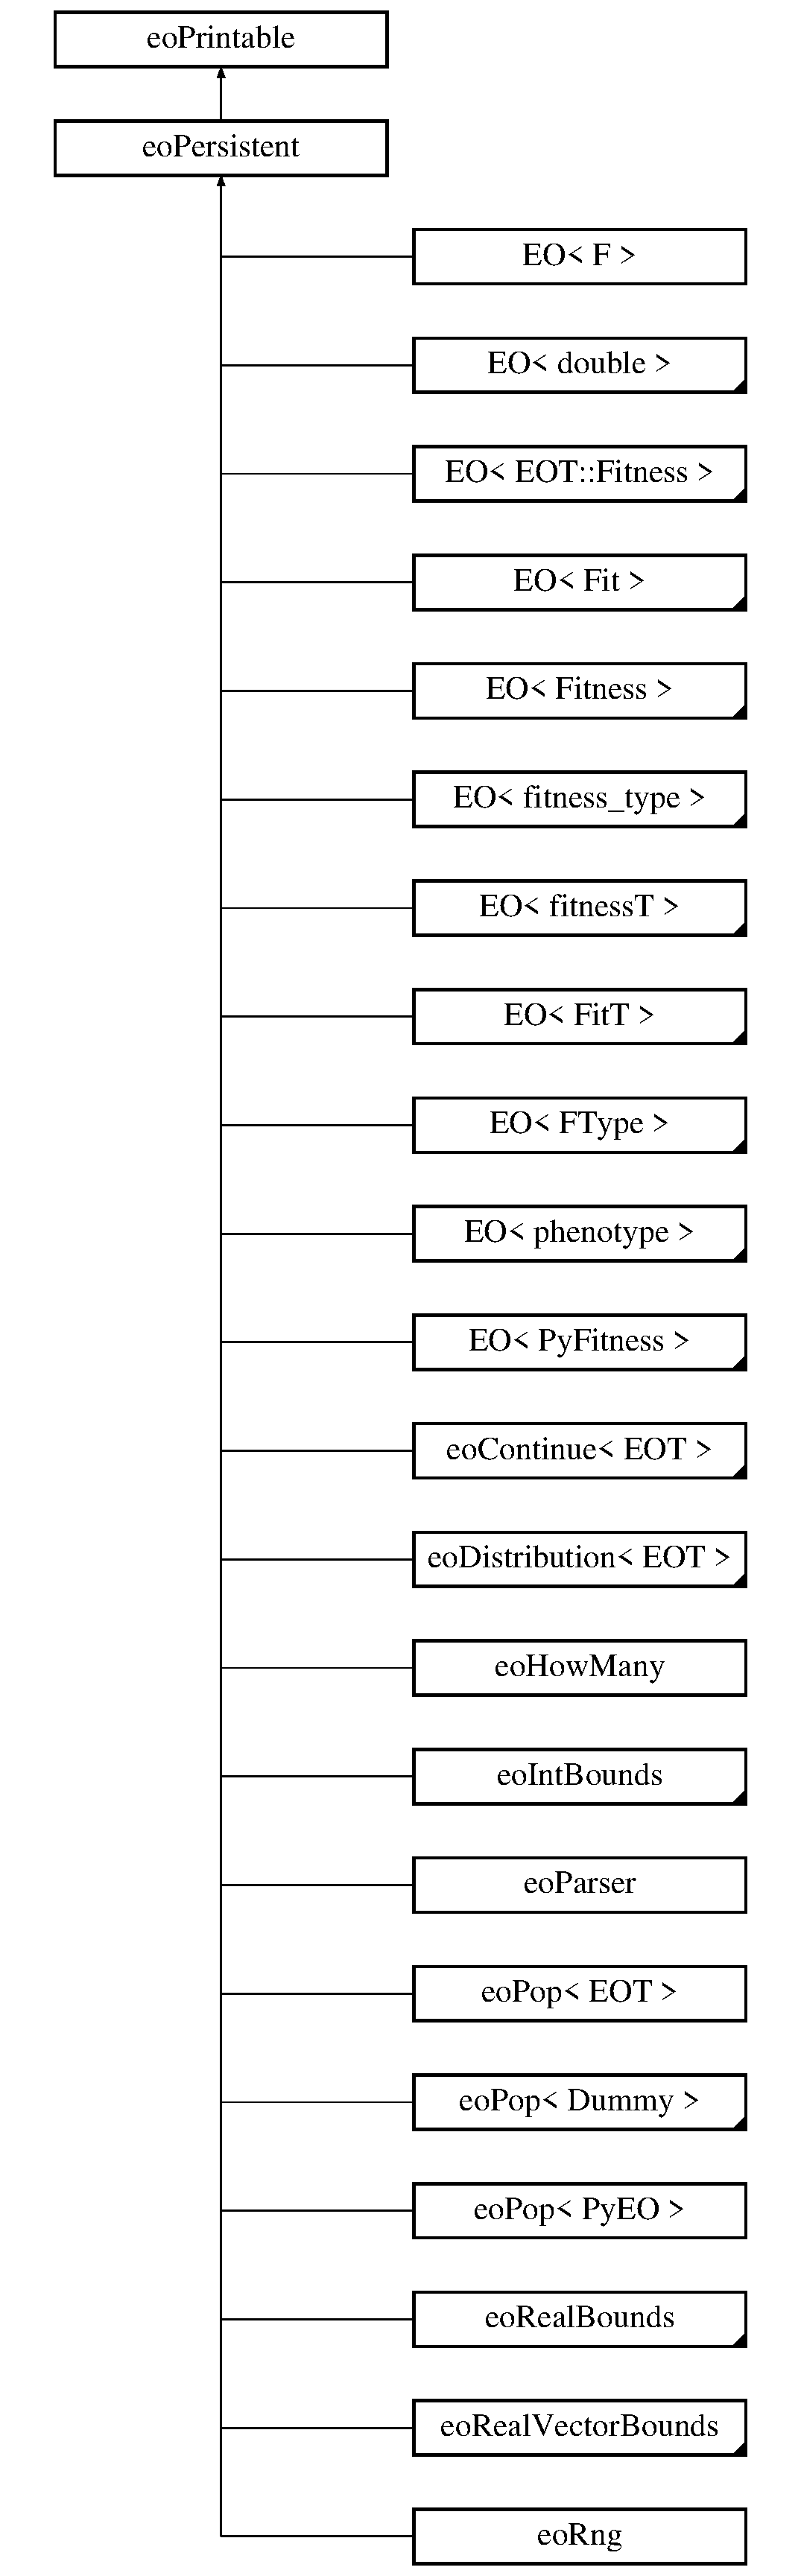
\includegraphics[height=12cm]{classeo_printable}
\end{center}
\end{figure}
\subsection*{Public Member Functions}
\begin{CompactItemize}
\item 
virtual {\bf $\sim$eo\-Printable} ()\label{classeo_printable_a0}

\begin{CompactList}\small\item\em Virtual dtor. They are needed in virtual class hierarchies. \item\end{CompactList}\item 
virtual void {\bf print\-On} (std::ostream \&\_\-os) const =0
\begin{CompactList}\small\item\em Write object. \item\end{CompactList}\end{CompactItemize}


\subsection{Detailed Description}
Base class for objects that can print themselves ({\bf print\-On}{\rm (p.\,\pageref{classeo_printable_a1})}\#). 

Besides, this file defines the standard output for all the objects; if the objects define print\-On there's no need to define \#operator $<$$<$\#.$\backslash$ This functionality was separated from {\bf eo\-Object}{\rm (p.\,\pageref{classeo_object})}, since it makes no sense to print some objects (for instance, a {\bf eo\-Factory}{\rm (p.\,\pageref{classeo_factory})}\# or a random number generator. 



Definition at line 43 of file eo\-Printable.h.

\subsection{Member Function Documentation}
\index{eoPrintable@{eo\-Printable}!printOn@{printOn}}
\index{printOn@{printOn}!eoPrintable@{eo\-Printable}}
\subsubsection{\setlength{\rightskip}{0pt plus 5cm}virtual void eo\-Printable::print\-On (std::ostream \& {\em \_\-os}) const\hspace{0.3cm}{\tt  [pure virtual]}}\label{classeo_printable_a1}


Write object. 

It's called print\-On since it prints the object on a stream. \begin{Desc}
\item[Parameters:]
\begin{description}
\item[{\em \_\-os}]A std::ostream. \end{description}
\end{Desc}


Implemented in {\bf EO$<$ F $>$} {\rm (p.\,\pageref{class_e_o_z10_2})}, {\bf eo\-Continue$<$ EOT $>$} {\rm (p.\,\pageref{classeo_continue_a2})}, {\bf eo\-Gen\-Continue$<$ EOT $>$} {\rm (p.\,\pageref{classeo_gen_continue_a7})}, {\bf eo\-Pop$<$ EOT $>$} {\rm (p.\,\pageref{classeo_pop_a18})}, {\bf eo\-Vector$<$ Fit\-T, Gene\-Type $>$} {\rm (p.\,\pageref{classeo_vector_a4})}, {\bf eo\-Es\-Full$<$ Fit $>$} {\rm (p.\,\pageref{classeo_es_full_a2})}, {\bf eo\-Es\-Simple$<$ Fit $>$} {\rm (p.\,\pageref{classeo_es_simple_a2})}, {\bf eo\-Es\-Stdev$<$ Fit $>$} {\rm (p.\,\pageref{classeo_es_stdev_a2})}, {\bf eo\-Bit$<$ Fit\-T $>$} {\rm (p.\,\pageref{classeo_bit_a2})}, {\bf eo\-PBILDistrib$<$ EOT $>$} {\rm (p.\,\pageref{classeo_p_b_i_l_distrib_a3})}, {\bf eo\-Parse\-Tree$<$ FType, Node $>$} {\rm (p.\,\pageref{classeo_parse_tree_a5})}, {\bf eo\-External\-EO$<$ Fit, External $>$} {\rm (p.\,\pageref{classeo_external_e_o_a4})}, {\bf eo\-String$<$ fitness\-T $>$} {\rm (p.\,\pageref{classeo_string_z24_1})}, {\bf eo\-How\-Many} {\rm (p.\,\pageref{classeo_how_many_a5})}, {\bf eo\-Int\-No\-Bounds} {\rm (p.\,\pageref{classeo_int_no_bounds_a14})}, {\bf eo\-Int\-Interval} {\rm (p.\,\pageref{classeo_int_interval_a15})}, {\bf eo\-Int\-Below\-Bound} {\rm (p.\,\pageref{classeo_int_below_bound_a15})}, {\bf eo\-Int\-Above\-Bound} {\rm (p.\,\pageref{classeo_int_above_bound_a15})}, {\bf eo\-General\-Int\-Bounds} {\rm (p.\,\pageref{classeo_general_int_bounds_a18})}, {\bf eo\-Parser} {\rm (p.\,\pageref{classeo_parser_a3})}, {\bf eo\-Real\-No\-Bounds} {\rm (p.\,\pageref{classeo_real_no_bounds_a13})}, {\bf eo\-Real\-Interval} {\rm (p.\,\pageref{classeo_real_interval_a14})}, {\bf eo\-Real\-Below\-Bound} {\rm (p.\,\pageref{classeo_real_below_bound_a14})}, {\bf eo\-Real\-Above\-Bound} {\rm (p.\,\pageref{classeo_real_above_bound_a14})}, {\bf eo\-General\-Real\-Bounds} {\rm (p.\,\pageref{classeo_general_real_bounds_a17})}, {\bf eo\-Real\-Vector\-Bounds} {\rm (p.\,\pageref{classeo_real_vector_bounds_a9})}, {\bf eo\-Rng} {\rm (p.\,\pageref{classeo_rng_a16})}, {\bf Dummy} {\rm (p.\,\pageref{struct_dummy_a1})}, {\bf Dummy} {\rm (p.\,\pageref{struct_dummy_a2})}, {\bf Dummy} {\rm (p.\,\pageref{struct_dummy_a3})}, {\bf Dummy} {\rm (p.\,\pageref{struct_dummy_a4})}, {\bf EO$<$ double $>$} {\rm (p.\,\pageref{class_e_o_z10_2})}, {\bf EO$<$ EOT::Fitness $>$} {\rm (p.\,\pageref{class_e_o_z10_2})}, {\bf EO$<$ Fit\-T $>$} {\rm (p.\,\pageref{class_e_o_z10_2})}, {\bf EO$<$ phenotype $>$} {\rm (p.\,\pageref{class_e_o_z10_2})}, {\bf EO$<$ fitness\-T $>$} {\rm (p.\,\pageref{class_e_o_z10_2})}, {\bf EO$<$ Fit $>$} {\rm (p.\,\pageref{class_e_o_z10_2})}, {\bf EO$<$ FType $>$} {\rm (p.\,\pageref{class_e_o_z10_2})}, {\bf EO$<$ fitness\_\-type $>$} {\rm (p.\,\pageref{class_e_o_z10_2})}, {\bf EO$<$ Fitness $>$} {\rm (p.\,\pageref{class_e_o_z10_2})}, {\bf EO$<$ Py\-Fitness $>$} {\rm (p.\,\pageref{class_e_o_z10_2})}, {\bf eo\-Pop$<$ Py\-EO $>$} {\rm (p.\,\pageref{classeo_pop_a18})}, {\bf eo\-Pop$<$ Dummy $>$} {\rm (p.\,\pageref{classeo_pop_a18})}, {\bf eo\-Vector$<$ Fit, double $>$} {\rm (p.\,\pageref{classeo_vector_a4})}, {\bf eo\-Vector$<$ Fit\-T, double $>$} {\rm (p.\,\pageref{classeo_vector_a4})}, and {\bf eo\-Vector$<$ Fit\-T, bool $>$} {\rm (p.\,\pageref{classeo_vector_a4})}.

Referenced by eo\-Real\-Vector\-Bounds::print\-On(), eo\-General\-Real\-Bounds::print\-On(), eo\-General\-Int\-Bounds::print\-On(), and eo\-State::save().

The documentation for this class was generated from the following file:\begin{CompactItemize}
\item 
eo\-Printable.h\end{CompactItemize}
